\subsection{Aplicación web}

Para realizar pruebas unitarias a la aplicación web desarrollado con Django se utilizo la herramienta que permite analizar que partes del código de un programa se están ejecutando y con ello determinar que bloques de código se deben de someter a pruebas.

Al utilizar coverage.py sobre el proyecto de Django se obtuvieron los resultados que se muestran en la figura \ref{fig:coverage}. El reporte que coverage.py arroja muestra la cantidad de código que se tiene que probar, el código que falta por probar, el excluido y el que se tienen cubierto con las pruebas.

Se logro cubrir el 100\% del código y se excluyeron algunas partes debido a que forman parte de los archivos de configuración de Django y porque fueron pruebas complicadas de elaborar.

\begin{figure}[h]
	\centering
	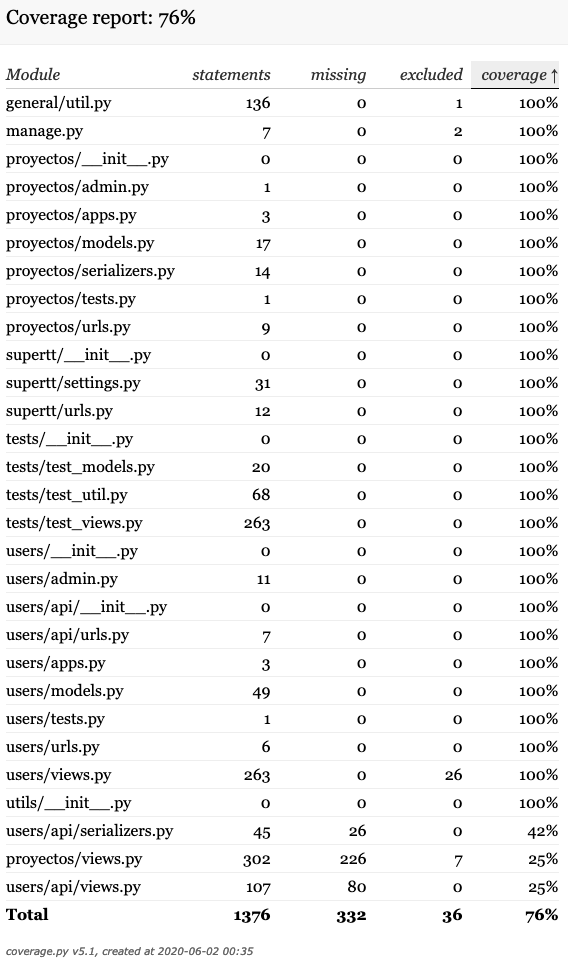
\includegraphics[width=450px]{capitulo6/unitarias/img/coverage.png}
	\caption{Reporte del código sometido a pruebas}
	\label{fig:coverage}
\end{figure}

Para realizar pruebas sobre estos bloques de código encontrados, se utilizo el módulo de pruebas unitarias con el que cuenta Django y se realizaron pruebas sobre los modelos, vistas y las clases de utilitaria que se desarrollaron.

\subsubsection{Pruebas sobre los modelos}

Un ejemplo de las pruebas sobre modelos es el siguiente código, en el cual se prueba el modelo del usuario y en cada uno de los métodos que comienzan con la palabra test determinan los diferentes casos de prueba a elaborar.

\subsubsection{Pruebas sobre los vistas}
\subsubsection{Pruebas sobre las clases de utilitaria}
